\documentclass[sigconf]{acmart}

\usepackage{amssymb}
\usepackage{amsmath}
\usepackage{amsfonts}
\usepackage{graphicx}
\usepackage{url}
\usepackage{xspace}
\usepackage{listings}
\usepackage[noline]{algorithm2e}
\usepackage{comment}
\usepackage{color}
\usepackage{multirow}
\usepackage{balance}
\usepackage{framed}
\usepackage{alltt}
\usepackage{xcolor}


% TODO
% copyright
%\setcopyright{acmlicensed}
%\setcopyright{rightsretained}


% TODO
%\acmDOI{10.475/123_4}

% TODO
%\acmISBN{123-4567-24-567/08/06}

% TODO
%\acmConference[WOODSTOCK'97]{ACM Woodstock conference}{July 1997}{El Paso, Texas USA}
%\acmYear{2018}
%\copyrightyear{2018}

% TODO
%\acmArticle{4}
%\acmPrice{15.00} 



% configures style of source code listings
\lstset{
	basicstyle=\small\sffamily
	%basicstyle=\scriptsize\ttfamily
	%numbers=left
}

\lstdefinelanguage{java}{
	morekeywords={abstract,continue,for,new,switch,assert,default,goto,package,synchronized,boolean,stream,event,filter,when,do,if,private,this,break,double,implements,protected,throw,byte,else,import,public,throws,case,enum,instanceof,return,transient,catch,extends,int,short,try,char,final,interface,static,void,class,finally,long,strictfp,volatile,const,float,native,super,while},
	sensitive=false,
	morestring=[b]",
	morestring=[b]',
	morecomment=[l]{//},
	morecomment=[s]{/*}{*/)},
	escapeinside=??,
	moredelim=[is][\textit]{__}{__},
	moredelim=[is][\textbf]{_*}{*_}
}
\lstnewenvironment{displayjava}
	{\lstset{language=java,basicstyle=\small\sffamily,tabsize=2,columns=fullflexible,captionpos=b,xleftmargin=1em,xrightmargin=1em}}{}
\lstnewenvironment{java}
	{\lstset{language=java,basicstyle=\small\sffamily,tabsize=2,columns=fullflexible,captionpos=b}}{}


\newcommand{\code}[1]{{\sf \small #1}\xspace}

\newcommand{\mi}[1]{\mathit{#1}}
\newcommand{\mr}[1]{\mathrm{#1}}
\newcommand{\mt}[1]{\mathtt{#1}}

\newcommand{\todo}[1]{{\bfseries TODO #1}}

% for writing comments
\newcommand{\PP}[1]{\textcolor{blue}{\bfseries PP: #1}} % Pavel Parizek
\newcommand{\PV}[1]{\textcolor{red}{\bfseries PV: #1}} % Premek Vysoky
\newcommand{\JB}[1]{\textcolor{orange}{\bfseries JB: #1}} % JetBrains

% coloring and font style commands
  % ANTLR
\newcommand{\antlrap}{\textquotesingle}
\newcommand{\antlrparserrule}[1]{\textcolor{blue}{#1}}
\newcommand{\antlrlexerrule}[1]{\textcolor{red}{#1}}
\newcommand{\antlrliteralnoap}[1]{\textcolor{brown}{#1}}
\newcommand{\antlrliteral}[1]{\antlrap\antlrliteralnoap{#1}\antlrap}
\newcommand{\antlrregex}[1]{\textcolor{olive}{#1}}
  % MPS in general
\newcommand{\mpsconcept}[1]{\textcolor{olive}{#1}}
\newcommand{\mpsinterface}[1]{\textcolor{violet}{#1}}
  % MPS structure
\newcommand{\mpsstkeyword}[1]{\textcolor{blue}{\textbf{#1}}}
\newcommand{\mpsstalias}[1]{\textcolor{olive}{\textbf{#1}}}
\newcommand{\mpsstproperty}[1]{\textcolor{violet}{\textbf{#1}}}
\newcommand{\mpsstplaceholder}[1]{\textcolor{gray}{\textbf{#1}}}
\newcommand{\mpsstcardinality}[1]{\textcolor{cyan}{\textbf{#1}}}
  % MPS editor
\newcommand{\mpsedkeyword}[1]{\textcolor{black}{\textbf{#1}}}
\newcommand{\mpsedtarget}[1]{\textcolor{magenta}{\textbf{#1}}}
\newcommand{\mpsedannotation}[1]{\textcolor{gray}{\textbf{#1}}}
  % MPS textgen
\newcommand{\mpstgkeyword}[1]{\textcolor{blue}{\textbf{#1}}}
\newcommand{\mpstgtarget}[1]{\textcolor{magenta}{\textbf{#1}}}
\newcommand{\mpstgparam}[1]{\textcolor{violet}{\textbf{#1}}}
\newcommand{\mpstgaction}[1]{\textcolor{violet}{\textbf{#1}}}
\newcommand{\mpstgliteral}[1]{\textcolor{olive}{\textbf{#1}}}
\newcommand{\mpstgnodeprop}[1]{\textcolor{darkgray}{\textbf{#1}}}



\begin{document}


\title{INGRID: Creating Languages in MPS from ANTLR Grammars}


\author{P\v{r}emysl Vysok\'y}
\affiliation{
  \institution{Charles University, Faculty of Mathematics and Physics}
  \city{Prague}
  \country{Czech Republic}
}
\email{premek.vysoky@gmail.com}

\author{Pavel Par\'izek}
\affiliation{
  \institution{Charles University, Faculty of Mathematics and Physics}
  \city{Prague}
  \country{Czech Republic}
}
\email{parizek@d3s.mff.cuni.cz}

\author{V\'aclav Pech}
\affiliation{
  \institution{JetBrains}
}
\email{vaclav@jetbrains.com}



\begin{abstract}
JetBrains MPS is a language workbench, an IDE that allows developers both to write code and create language definitions.
It leverages the concept of projectional editing, where the developer directly manipulates the AST representation of program code.
While MPS focuses on domain-specific languages (DSL), it needs to support also general-purpose programming languages (GPPLs) --- for example, to compile and run programs written in some DSL.
%, or to enable combination of GPPLs with DSLs created in MPS.

We present \textsc{Ingrid}, a method for construction of a language definition in MPS based on its ANTLR grammar.
The structure of a language is generated automatically, but its projectional editor and other aspects has to be adjusted manually.
%by the user.
During the development of \textsc{Ingrid}, we encountered several challenges related to the mapping between grammars and language definitions in MPS that are based on object-oriented principles.
Another difficulty is that grammars do not hold any information about code layout.

We implemented \textsc{Ingrid} as a plugin for MPS and evaluated it on several mainstream GPPLs, such as JavaScript and C\#.
Results show that our approach is practical, and it saves the user from many hours of tedious and error-prone work.
Necessary manual adjustments take only a short time.
\end{abstract}


\begin{CCSXML}
<ccs2012>
<concept>
<concept_id>10011007.10011006.10011008.10011009.10011019</concept_id>
<concept_desc>Software and its engineering~Extensible languages</concept_desc>
<concept_significance>500</concept_significance>
</concept>
<concept>
<concept_id>10011007.10011006.10011041.10011047</concept_id>
<concept_desc>Software and its engineering~Source code generation</concept_desc>
<concept_significance>500</concept_significance>
</concept>
<concept>
<concept_id>10011007.10011006.10011041.10011688</concept_id>
<concept_desc>Software and its engineering~Parsers</concept_desc>
<concept_significance>500</concept_significance>
</concept>
<concept>
<concept_id>10011007.10011006.10011066.10011069</concept_id>
<concept_desc>Software and its engineering~Integrated and visual development environments</concept_desc>
<concept_significance>500</concept_significance>
</concept>
</ccs2012>
\end{CCSXML}

\ccsdesc[500]{Software and its engineering~Extensible languages}
\ccsdesc[500]{Software and its engineering~Source code generation}
\ccsdesc[500]{Software and its engineering~Parsers}
\ccsdesc[500]{Software and its engineering~Integrated and visual development environments}

\keywords{language workbench, projectional editor, grammar, domain-specific language, ANTLR, JetBrains MPS}

\maketitle



\section{Introduction}

The prevailing approach to define valid syntaxes for programming languages is through grammars, which are typically written in notations based on the Extended Backus-Naur Form (EBNF).
Many popular tools exist for automated generation of parsers from the grammar definitions --- for example, ANTLR~\cite{ref:ANTLRBOOK,ref:ANTLR} and Bison/Flex~\cite{ref:BISONFLEX}.
The source code of programs is written in a text editor, usually embedded into an IDE. Parsers are used to create an abstract syntax tree (AST) representation of the code, e.g. inside the compiler.

An alternative approach is projectional (or structural) editing, where a developer directly manipulates the AST representation of the source code instead of plain text.
This idea emerged as early as in 1970s, but it failed to get adopted widely, mostly due to inconvenient and unnatural way of manipulating code.
A recent revival of projectional editing has been observed in the area of language workbenches --- IDE-like tools that enable the developers to manipulate the actual language definition.
The Meta Programming System (MPS)~\cite{ref:MPS} by JetBrains is an open-source language workbench that focuses on domain specific languages (DSL) and leverages the concept of projectional editing.
MPS provides the whole IDE infrastructure that enables developers to design custom languages, use them to write program code, and compile the code into executables.
We provide more technical details about MPS in Section~\ref{sect:MPS}.
In the rest of the paper, we will use MPS to illustrate the general concepts and issues that apply also to other language workbenches.

%MPS has put extra effort into making text manipulation feel like editing real text.
%MPS models, although being persisted as XML or binary files, can be versioned using the industry standard source-control systems (Git, Subversion).
%On-line model browsers have been incorporated into some of the popular public source code repositories (BitBucket) [reference] .

Projectional editing, keeping the code in the AST form, and in particular the absence of parsers, brings along several benefits.
\begin{itemize}
	\item The developers practically cannot enter syntactically invalid code, because a projectional editor controls the interaction between the user and the code. An AST created by the editor can represent only a syntactically valid code.
	\item Programming languages can be defined in a modular way, and multiple languages can be easily combined together or one can extend another, while parsers seriously limit language modularity for traditional parsed languages.
	\item The languages may support contextual or non-parseable notations, such as tables, diagrams and positional syntax.
	\item Since the projection is detached from the physical representation of code (AST), authors of languages can define multiple notations and allow the developers to switch between different representations of the code on the screen.
\end{itemize}
All of this is useful especially for DSLs, which are frequently used by domain experts who may not be professional software developers.
The mbeddr project~\cite{ref:MBEDDR}, which extends C with numerous domain-specific constructs and data types, illustrates the abilities of language workbenches in general and of MPS in particular.

On the other hand, the usage of projectional editors introduces some new problems.
Before a language can be used inside MPS, it has to be defined in a special way through the MPS infrastructure, so that the IDE can understand the language and work with it.
Specifically, an author of a language has to create:
\begin{enumerate}
	\item the abstract syntax called \emph{Structure}, which defines the types of allowed AST nodes,
	\item the concrete syntax called \emph{Editor}, i.e. projection of the AST on the screen and its interactions with the user, and
	\item text generation scripts, also called \emph{TextGen}, to enable creation of plain text files used as input for compilers.
\end{enumerate}	
Again, we provide additional technical details in Section~\ref{sect:MPS}.

MPS is typically used for syntactically rich DSLs, which are likely to benefit most from overcoming the limitations of parser-based languages.
Before a program written in such a DSL can be executed, it is transformed on the AST level by a series of model-to-model transformations to an AST model that represents the desired semantics in a general-purpose language (GPL), such as C or Java.
This model is then converted to a textual representation of that language and compiled by the standard means of the target platform.
Therefore, the target GPL must also be defined by the MPS means in order to allow the DSLs to have their models transformed into a model in the GPL.

However, very few mainstream GPLs are now fully supported by MPS, because it requires substantial effort to manually create a full definition of a GPL in MPS.
Only Java and C have been implemented to date, which limits the authors of DSLs to only target these supported GPLs.
The overall goal of our project is to automatize the process of language definition in MPS as much as possible, exploiting the fact that a big part of this process is quite straightforward.
We believe that such an automated process would encourage and speed-up the migration of more GPLs into MPS, thus giving the authors of DSLs more options.
Other possible applications include the support for writing programs in GPLs using the projectional editor and combination of GPLs with domain-specific languages natively created in MPS.

In this paper we present INGRID, a method and a tool for semi-automated construction of the definition of a programming language in MPS that uses an ANTLR grammar of the language as a description of its syntax.
We discuss the main challenges that we encountered during the development of INGRID and our solution to them.
Although we explain everything on the examples of MPS languages and ANTLR grammars, we emphasize that most of the challenges are general. 
They apply to the relation between the two approaches to the definition of a programming language --- (i) one that uses grammars in an EBNF-like notation, with rules and tokens written in plain text, and the corresponding parser generators, and (ii) the structured object-oriented approach used in MPS and other language workbenches.
Specifically, the description of a language in the form of a grammar does not hold any information about the code layout, and the grammar typically contains many rules that do not directly correspond to AST nodes and programming language constructs.
We provide more details in Section~\ref{sect:LANGDEF}.

The INGRID tool can help also to make the construction of DSLs more efficient.
Based on our experience, we believe that, especially for simple languages, it is less time consuming to write their grammar by hand and then create the language definition in MPS using INGRID, than to create the language manually using the MPS GUI.

%INGRID allows developers to leverage all the features that MPS has to offer together with general purpose languages such as C++, JavaScript or Python.

The rest of the paper has the following structure.
In the next section, we provide necessary information about MPS and a brief overview of projects with similar goals as INGRID.
Then, in Section~\ref{sect:LANGDEF}, we describe our approach to the construction of a language definition in MPS from its ANTLR grammar, discussing the major challenges together with our solution along the way.
We also discuss our experience with usage of INGRID on complex mainstream languages, such as JavaScript and C\#, and highlight open problems (Section~\ref{sect:EVAL}), and then we conclude.


\section{Background and Related Work}
\label{sect:BACKGRELWORK}

In this section, first we introduce basic features of the MPS platform, and then we discuss other existing projects that aim to add support for general purpose languages into MPS.

\subsection{JetBrains MPS}
\label{sect:MPS}

JetBrains MPS is a complete language workbench --- an integrated development environment that allows developers to create their own languages and use them to write code.
The code can then be transformed into a target language, typically a GPL, such as Java or C, and eventually compiled into executable programs.

As we already indicated, MPS differs from typical IDEs in one important aspect --- the projectional editor.
The developer does not work with the textual representation of the source code directly, but rather with its AST that is the model of the code.
Basically, when using the MPS projectional editor, programs are created by assembling the tree (AST) out of predefined building blocks of selected languages.
The definition of a language in MPS dictates, where in the AST can certain elements be placed and how they can be nested inside other elements.
On the other hand, in traditional IDEs it is the parser that constructs an AST of a program using the language's elements.

The building blocks of MPS models are called nodes.
Code of any program in MPS is built from nodes, which represent instances of concepts defined in one of the languages that the program declares to be using.
In the context of MPS, a concept is, in fact, a building block of a language definition.
We use the terms \emph{MPS concept} and \emph{AST node} when needed to avoid confusion.

One of the key advantages of projectional editing stems from the separation of abstract and concrete syntax.
While AST provides a complete and precise representation of the code, the way it is displayed on the screen and the way the user interacts with it are unconstrained.
The editor can take any visual form and shape.
The language author can define multiple alternative visualizations and let the developer choose one that fits best the task at hand --- for example, editing, debugging, reviewing, resolving merge conflicts, etc.
In particular, the visual representations are not bound to be just textual at all.
For example, blocks corresponding to branches of an \code{if-then-else} statement can be aligned next to each other and displayed with different background colors.

The definition of an MPS concept (language element) consists of several aspects, where each aspect codifies a different part of the AST nodes' behavior.
The essential aspects are the following: \emph{Structure} (abstract syntax), \emph{Editor} (concrete syntax) and \emph{TextGen}.
Editor defines the concrete syntax (i.e., how the code is visualized and edited) and TextGen specifies how AST nodes are transformed into textual representation.
If, instead of generating text directly, programs in the language are supposed to be transformed into another language that is available in MPS, the Generator aspect must be used to specify the model-to-model transformation rules.
Since only the Structure, Editor and TextGen aspects are relevant for the contribution of this paper, we describe these three below in more detail, and neglect other aspects such as type system and data-flow.

Languages are built from the concepts using techniques known from object-oriented programming --- containment, inheritance, interfaces, and so on.
Therefore, a definition of a whole language in MPS typically has an object-oriented and hierarchical nature.

\paragraph{Structure.}
The fundamental aspect of any MPS language is Structure.
It must be created first for each intended element (concept) of the language.
Structure specifies core attributes of an MPS concept such as the name, inheritance relationships, possible child concepts (including their types and cardinalities), the implemented interfaces, and references to other AST nodes.
% other properties (fields of any type that can hold values), etc.
Figure~\ref{fig:if_statement_structure} shows definition of the Structure aspect for the \code{if-else} statement.

The definition of Structure restricts the type of AST nodes that can appear at a particular place in the tree.
For example, one can restrict the condition in the \code{if-then-else} statement to be a boolean expression, and the \code{then}-block to be a list of statements.

\begin{figure}[ht]
\centering
\begin{alltt}
\small
\mpsstkeyword{concept} IfStatement \mpsstkeyword{extends} Statement
        \mpsstkeyword{implements} IContainsStatementList
                   IDontSubstituteByDefault
                   IConditional

  \mpsstkeyword{instance can be root:} false
  \mpsstkeyword{alias:} \mpsstalias{if}
  \mpsstkeyword{short description:} \mpsstplaceholder{<no short description>}

  \mpsstkeyword{properties:}
  \mpsstproperty{forceOneLine}   : boolean
  \mpsstproperty{forceMultiLine} : boolean
  
  \mpsstkeyword{children:}
  \mpsstproperty{condition}        : Expression[\mpsstcardinality{1}]
  \mpsstproperty{ifFalseStatement} : Statement[\mpsstcardinality{0..1}]
  \mpsstproperty{ifTrue}           : StatementList[\mpsstcardinality{1}]
  \mpsstproperty{elsifClauses}     : ElsifClause[\mpsstcardinality{0..n}]
  
  \mpsstkeyword{references:}
  \mpsstplaceholder{<< ... >>}
\end{alltt}
\caption{Structure aspect of the \code{if-else} statement}
\label{fig:if_statement_structure}
\end{figure}

\paragraph{Editor.}
The Editor aspect is where the language designer specifies what the projectional editor representation of a code fragment (an AST) looks like on the screen and how the user interacts with the code.
JetBrains have developed a cellular system that enables placing properties and children of a node (concept) into different cells.
The author usually incorporates all of the node's children, references, and properties inside the representation, so that the future users of the language can insert all values that the node expects.
Additionally, cells of the editor can be styled using a language similar to CSS.
The supported visual characteristics include text color and indentation.

Figure~\ref{fig:if_editor_definition} shows an example of what the definition of the Editor aspect for the \code{if-else} statement might look like.
While here we indicate positions of cell borders on each line by spaces (just for the purpose of illustration), MPS GUI actually uses a graphically much more appealing way of displaying the Editor aspects, which involves vertical and horizontal lines of different colors and also background colors other than white for some cells.
The symbols \verb|[-| and \verb|-]| represent layout information (cells), which define rules for mutual positioning of the contained cells (vertical, horizontal, indentation).

\begin{figure}[ht]
\centering
\begin{alltt}
\small
\mpsedannotation{<default>} \mpsedkeyword{editor for concept} \mpsedtarget{IfStatement}
  \mpsedkeyword{node cell layout:}
    [-
      \mpsedkeyword{if} \textbf{(} \% conditions \% \textbf{)} [-
      \textbf{\{}
      [- \% ifTrue % -]
      \textbf{\}}
    -]
    ?[- \mpsedkeyword{else} \% ifFalseStatement \% -]
    -]
\end{alltt}
\caption{Editor aspect for the \code{if-else} statement}
\label{fig:if_editor_definition}
\end{figure}

\paragraph{BaseLanguage.}
Another important feature of MPS that we need to describe in more detail is \emph{BaseLanguage}~\cite{ref:BASELANG}.
It is a clone of Java implemented using the MPS constructs.
BaseLanguage was developed in the early days of MPS in order to implement MPS itself and also to support the basic set of language-definition DSLs,
Although BaseLanguage is syntactically almost identical to Java, it is edited in a projectional editor, just like all the languages in MPS.
The language-definition DSLs, used to define custom languages by their authors, are generated into the BaseLanguage.
Similarly, all the custom DSLs that are meant to be generated into Java choose BaseLanguage as their generation target.
The conversion to textual Java is handled by BaseLanguage without any further manual effort, since BaseLanguage has a TextGen aspect defined, which translates BaseLanguage code into textual Java sources.

\paragraph{TextGen.}
The TextGen aspect specifies how a given AST node will be translated into plain text representation.
It is typically needed only for the bottom-line base languages.
DSLs, on the other hand, need to define rules for model-to-model conversions (Generators), since these are rarely converted to text directly.
After TextGen has generated textual sources from an AST, a compiler for the particular GPL is invoked to compile the textual sources into binary code.
The TextGen definition follows a very straightforward pattern --- each node outputs its textual representation into a buffer, while calling TextGen of its children nodes at the right moments.
MPS calls the corresponding method on the root AST nodes of the given program.

\begin{figure}[ht]
\centering
\begin{alltt}
\small
\mpstgkeyword{text gen component for concept} \mpstgtarget{IfStatement} \{
  \mpstgparam{(context, buffer, node)->void} \{
    \mpstgaction{append} \textcolor{Blue}{\textbf{\textbackslash{}n;}}
    \mpstgaction{indent buffer;}
    \mpstgaction{append} \{\mpstgliteral{if (}\} \$\{\mpstgparam{node}.\mpstgnodeprop{condition}\} \{\mpstgliteral{) \{}\};
    \mpstgkeyword{with indent} \{
      \mpstgaction{append} \$\{\mpstgparam{node}.\mpstgnodeprop{ifTrue}\};
    \}
    \mpstgaction{append} \textcolor{Blue}{\textbf{\textbackslash{}n}} \{\mpstgliteral{\}}\} \$list\{\mpstgparam{node}.\mpstgnodeprop{elsifClauses}\};
    \mpstgkeyword{if} (\mpstgparam{node}.\mpstgnodeprop{ifFalseStatement}.\textbf{isNotNull}) \{
      \mpstgaction{append} \{ \mpstgliteral{else}\} \$\{\mpstgparam{node}.\mpstgnodeprop{isFalseStatement}\};
    \}
  \}
\}
\end{alltt}
\caption{TextGen aspect definition for the \code{if-else} statement}
\label{fig:if_statement_textgen}
\end{figure}

TextGen aspect for each AST node (concept of the language) has to be defined using the BaseLanguage.
Again, we include an example for the \code{if-else} statement (Figure~\ref{fig:if_statement_textgen}).

\subsection{Related Projects}
\label{sect:RELATED}

The BaseLanguage~\cite{ref:BASELANG} is an almost full port of the Java language, extended with MPS-specific features.
It was created manually by JetBrains, and it is still undergoing changes as Java itself is evolving.

The C language has also been manually tailored for MPS within the mbeddr project~\cite{ref:MBEDDR}.

Besides that, we are aware of three other projects that provide certain support for GPLs in the context of MPS --- namely PE4MPS, ANTLR{\_}MPS, and mps-metabnf.
We describe their main features and limitations in this section.

\paragraph{PE4MPS.}
PE4MPS~\cite{ref:PE4MPS} is a project that addresses the lack of information about code layout in grammars by using so called PE grammars~\cite{ref:PE}, which is a new grammar notation proposed by the same author.
The abbreviation PE stands for projectional editing.

PE grammars extend the syntax of the ANTLR v4 notation by custom constructs that provide information about the possible layout of AST nodes.
The current version, as of November 2016, supports just horizontal lists, vertical lists, and some indentation rules.
However, even these few features make the already complex syntax of ANTLR v4 much more complicated.

The PE4MPS tool creates an MPS language in a single atomic step.
An input PE file is loaded and processed by the PE parser, and then all concepts (AST nodes) and their aspects are directly generated inside MPS.
Information about the code layout, extracted from the PE file, is used when generating the projectional editor for every AST node.

The main disadvantage of the PE4MPS approach is that it only shifts the tedious manual work from creating projectional editors in the MPS IDE to writing PE grammars in plain text.
In particular, language developers are forced to specify the code layout manually in PE grammars, through the corresponding extensions.
Usage of a standard text editor is inferior (and much more error-prone) with respect to MPS, which has been designed for the purpose of specifying the code layout and provides lot of support to developers.
Another limitation of PE4MPS is that it does not implement the full ANTLR syntax.
Every grammar might require non-trivial adjustments before it can be processed using the PE4MPS tool.
To compare, the goals behind our INGRID approach are (1) to enable import of as many languages as possible out-of-the-box with maximal automation and (2) to adopt the full specification of every imported language.

\paragraph{ANTLR{\_}MPS.}
The ANTLR{\_}MPS project~\cite{ref:ANTLR2MPS} also uses the ANTLR v4 grammar notation, but otherwise works quite differently from PE4MPS.
We provide only a brief mention here because this project is in an early stage of development.
Its author created an ANTLRv4 MPS language, which captures the syntax of ANTLRv4 notation using MPS concepts.
Given some language as input, the textual grammar of the language is imported automatically into MPS, taking the form of the ANTLRv4 MPS language.
The next step would be to create a new MPS language from the grammar definition in MPS, but it is not implemented yet.

However, the project has also other important limitations.
The tool does not generate any parent-child relationships in the Structure aspect, and it provides no support for the projectional editor at all (by completely neglecting the Editor and TextGen aspects).

\paragraph{mps-metabnf.}
The mps-metabnf tool~\cite{ref:MPSMETABNF}, implemented by members of the DSLFoundry group, builds upon similar ideas as the ANTLR{\_}MPS project described above.
Authors of this project, too, created an MPS language that can be used to capture ANTLR grammars.
Every imported grammar is represented using this ANTLRv4 MPS language.
A user is then able to adjust the grammar as he wishes, specifying the code layout in the projectional editor.
In the last step, the target MPS language is derived from the adjusted grammar definition.

The main limitation of this approach is the need to perform the last step manually, because MPS currently does not provide any support for automated transformation of a grammar captured by the ANTLRv4 MPS language into the definition of the actual target MPS language.


\section{Creating Language Definition in MPS}
\label{sect:LANGDEF}

The proposed \textsc{Ingrid} method accepts grammars in the ANTLR v4 notation~\cite{ref:ANTLRBOOK} as input.
All widely used programming languages have their syntax defined using this notation~\footnote{https://github.com/antlr/grammars-v4}.
Unlike some of the related projects, we did not extend the notation with any custom features, and we also did not create an MPS language for the ANTLR notation.

The process of MPS language construction, as performed by \textsc{Ingrid}, consists of four phases --- the first is parsing of the input grammar, which is followed by definition of the essential aspects of the language (Structure, Editor, and TextGen).
Each of the phases 2-4 is exclusively and fully responsible for one aspect.

\textsc{Ingrid} is currently able to create (i) a full Structure aspect for each element (type of an AST node) of the given language, (ii) a very basic Editor, and (iii) a basic TextGen aspect.
Therefore, the resulting MPS language typically still has to be adjusted manually to improve its usability, and the human users must also define the remaining aspects not yet supported by \textsc{Ingrid}.

Our approach differs from the related projects (Section~\ref{sect:RELATED}) especially in the level of automation. It also has much better support for the definition of Editor and TextGen.

\subsection{Running Example}

We will describe the \textsc{Ingrid} method using the example of a simplified XML language that is defined in Figure~\ref{fig:SIMPLEXML}.
The \emph{SimpleXML} language is small but complex enough to be used for illustration of the main challenges and behavior of the proposed algorithms.

\begin{figure*}[ht]
\centering
\begin{framed}
\begin{alltt}
\textbf{grammar} \textit{SimpleXML};
\antlrparserrule{document}  : \antlrparserrule{prolog}? \antlrparserrule{comment}? \antlrparserrule{element} ;
\antlrparserrule{prolog}    : \antlrliteral{<?xml } \antlrparserrule{attrib}* \antlrliteral{?>} ;
\antlrparserrule{comment}   : \antlrliteral{<!--} \antlrlexerrule{TEXT} \antlrliteral{-->} ;
\antlrparserrule{element}   : \antlrliteral{<} \antlrlexerrule{Name} \antlrparserrule{attrib}* \antlrliteral{>} \antlrparserrule{content}* \antlrliteral{</} \antlrlexerrule{Name} \antlrliteral{>} | \antlrliteral{<} \antlrlexerrule{Name} \antlrparserrule{attrib}* \antlrliteral{/>} ;
\antlrparserrule{attrib}    : \antlrlexerrule{Name} \antlrliteral{="} \antlrlexerrule{TEXT} \antlrliteral{"} ;
\antlrparserrule{content}   : \antlrlexerrule{TEXT} | \antlrparserrule{element} | \antlrparserrule{comment} | \antlrlexerrule{CDATA} ;
\antlrlexerrule{Name}      : \antlrlexerrule{NameStartChar} \antlrlexerrule{NameChar}* ;
\antlrlexerrule{DIGIT}     : \antlrregex{[0-9]} ;
\antlrlexerrule{NameChar}  : \antlrlexerrule{NameStartChar} | \antlrliteral{-} | \antlrliteral{\_} | \antlrliteral{.} | \antlrlexerrule{DIGIT} ;
\antlrlexerrule{NameStartChar} : \antlrregex{[:a-zA-Z]} ;
\antlrlexerrule{TEXT}      : \antlrregex{~[<"]*} ;
\antlrlexerrule{CDATA}     : \antlrliteral{<![CDATA[} \antlrregex{.*?} \antlrliteral{]]>} ;
\end{alltt}
\end{framed}
\caption{Grammar of the SimpleXML language in the ANTLR v4 notation}
\label{fig:SIMPLEXML}
\end{figure*}

The grammar of SimpleXML contains elements of the kinds that are listed below.
Each color in Figure~\ref{fig:SIMPLEXML} corresponds to a different kind in a way that is indicated by the list item headers.
\begin{itemize}
	\item \textbf{ANTLR v4 keywords} are required by the notation.
	\item \antlrparserrule{\textbf{Parser rules}} describe the structure of a language.
		Alternatives on the right side of a rule are separated by the pipe character ($|$).
	\item \antlrlexerrule{\textbf{Lexer rules}} describe terminal symbols that the parser matches against the input string.
		A terminal symbol can be encoded as a string value or using a regular expression.
	\item \antlrliteralnoap{\textbf{String literals}}, always written inside of a pair of single quote marks, also represent terminal symbols, but by exact match to a string constant.
	\item \antlrregex{\textbf{Regular expressions}} describe string tokens to be matched against regular expressions with a special ANTLR v4 regex notation\footnote{https://github.com/antlr/antlr4/blob/master/doc/lexer-rules.md}.
\end{itemize}
Elements on the right side of a rule can be annotated with standard EBNF operators (\code{?}, \code{+}, \code{*}) that specify the allowed number of occurrences.

\subsection{Phase 1: Parsing Input Grammar}

The first phase in the process of MPS language construction is parsing of the input ANTLR v4 grammar.
It is done using an ANTLR parser that was automatically generated from the grammar of the ANTLR v4 notation itself.
Nevertheless, the full AST, which comes out of the parser, is quite complex and contains information not relevant for the \textsc{Ingrid} algorithm.
In order to get a simple representation that is easy to process by the later phases and keeps only information necessary for the construction of MPS languages, several steps of post-processing of the AST are performed in this phase.
An output is a custom AST-like structure representing the grammar, especially the hierarchy of parser rules.

The representation of lexer rules (tokens) in the AST has to be simplified too.
Note that, in the ANTLR notation, lexer rules can be built from alternatives just like the parser rules --- see, for example, the lexer rule \antlrlexerrule{Name} from our SimpleXML language (Figure~\ref{fig:SIMPLEXML}).
For each lexer rule, the parser produces a tree that captures the structure of the rule.
However, the lexer rules are, in fact, just regular expressions used to recognize tokens in the input string.

Every tree that represents a lexer rule is flattened into the equivalent regular expression by the recursive algorithm specified in Figure~\ref{fig:ALGFLATTEN}.
A distinct sequence is created from the elements of each alternative, and then all those sequences are joined by the alternation operator \code{$|$} to form a regular expression.

\begin{figure}[ht]
\centering
\begin{framed}
\begin{alltt}
Flatten(\textit{R}):
  \textit{T} = empty list
  \textbf{for each} alternative \textit{A} \textbf{in} rule \textit{R}:
    \textit{R} = \antlrap\antlrap
    \textbf{for each} element \textit{E} \textbf{of} \textit{A}:
      \textbf{if} \textit{E} is not yet flattened \textbf{then}:
        Flatten(\textit{E})
      \textit{R}.append(\textit{E})
      \textit{R}.append(\textit{E}.operator)
    \textit{T}.add(\textit{R})
  build string S from elements of \textit{T}:
    \textit{S} = \(t\sb{1}\) | \(t\sb{2}\) | \(\ldots\) | \(t\sb{n}\)
  \textbf{return} \textit{S}
\end{alltt}
\end{framed}
\caption{Flattening algorithm}
\label{fig:ALGFLATTEN}
\end{figure}

The output of \texttt{Flatten(Name)}, i.e. application of the algorithm to the \antlrlexerrule{Name} rule, is this regular expression:

\begin{center}
  \texttt{[:a-zA-Z]([:a-zA-Z]|\textbackslash-|{\_}|\textbackslash.|[0-9])*}
\end{center}
It defines the syntactically valid identifiers of elements and attributes in SimpleXML.
Each identifier must begin with a letter, followed by any combination of letters, digits, underscore, dash, or a dot.

\subsection{Phase 2: Structure}

In the next phase, the complete structure of the MPS language is automatically generated from the AST that represents syntax of the input language.
Elements of the Structure aspect are derived from the AST nodes, and then linked appropriately.
Therefore, structure of the MPS language is usually similar to the original ANTLR grammar.

When designing the process for translating AST nodes (i.e., grammar rules) into the MPS language structure, we faced several challenges.
The main challenge related to the structure, as we already mentioned in the introduction, is that a grammar typically contains rules that do not directly correspond to programming language constructs.
Such rules exist at the intermediate layers of a syntax hierarchy.
Their main purpose is to enable easier understanding and maintenance of the grammar by humans.
However, presence of the intermediate layers significantly complicates usage of the given language in MPS, and the layers are actually not necessary for construction of an MPS language.
We show examples illustrating this problem, which we call a \emph{layer problem}, later in the subsection where we describe our solution.

As a part of the \textsc{Ingrid} method, we have designed an approach to eliminate the unnecessary layers during construction of the Structure aspect --- we call it the \emph{shortcut} approach (Section~\ref{sect:SHORTCUT}).
However, before focusing on the intermediate layers and the shortcut approach, we describe the basic principles of translation from the AST into the language structure.

In MPS, each concept of the language (i.e., every AST node) is represented by an object that may have a parent, some children, and properties of any data type.
Additionally, the object may implement any number of interfaces, and it may also contain references to objects representing other AST nodes.
The parent-child relationships between objects that make the Structure aspect are derived from rules of the grammar (i.e., from the structure of the AST).
For each rule, the object corresponding to the left-hand side is in the parent-child relationships with sets of objects that represent language elements referenced by the right-hand side.
If a rule has multiple alternatives, then a distinct object (MPS concept) has to be created in the structure for each alternative.
The name of a concept (object) in MPS is composed from (1) the name of the AST node, which is equivalent to the string encoding of the left-hand side of the corresponding rule, and (2) the number indicating the position of the respective alternative on the right-hand side of the rule.

\begin{figure}[ht]
\centering
\begin{alltt}
\small
\mpsstkeyword{concept} Element\_1 \mpsstkeyword{extends} BaseConcept
        \mpsstkeyword{implements} IContent, IElement

  \mpsstkeyword{instance can be root:} false
  \mpsstkeyword{alias:} \mpsstalias{< > </ >}
  \mpsstkeyword{short description:} \mpsstalias{Element}

  \mpsstkeyword{properties:}
  \mpsstproperty{Name\_1} : Name
  \mpsstproperty{Name\_2} : Name
  
  \mpsstkeyword{children:}
  \mpsstproperty{Attribute\_1} : Attribute[\mpsstcardinality{0..n}]
  \mpsstproperty{Content\_2}   : IContent[\mpsstcardinality{0..n}]
\end{alltt}
\caption{Structure aspect of the \code{Element{\_}1} concept}
\label{fig:ELEMENTSTRUCT}
\end{figure}

Consider the parser rule \antlrparserrule{element} from the grammar in Figure~\ref{fig:SIMPLEXML}.
Its first alternative represents the full XML element with content.
Figure~\ref{fig:ELEMENTSTRUCT} shows the Structure aspect for the MPS concept (object) named \code{Element{\_}1} that corresponds to the alternative.
The object contains two properties, one for each reference to the lexer rule \antlrlexerrule{Name}.
Values of these properties will be restricted using the regular expression that corresponds to the lexer rule \antlrlexerrule{Name}.
String literals, such as the opening and closing brackets (\antlrliteral{\textless}, \antlrliteral{/\textgreater}) in XML, are omitted because they will be defined only in the Editor aspect for this concept.

References to other parser rules are captured by pointers to child objects.
The types of child objects, such as \code{IContent} in the \code{Element{\_}1} concept, are determined as follows.
Consider the \antlrparserrule{content} rule from the SimpleXML language.
We show just the relevant fragment of the grammar again in Figure~\ref{fig:CONTENTRULE}.
An object corresponding to any one of the four alternatives could be the actual value anywhere the \antlrparserrule{content} rule is referenced.

\begin{figure}[ht]
\centering
\begin{alltt}
\small
\antlrparserrule{content} : \antlrlexerrule{TEXT} | \antlrparserrule{element} | \antlrparserrule{comment} | \antlrlexerrule{CDATA} ;
\end{alltt}
\caption{Parser rule \antlrparserrule{content}}
\label{fig:CONTENTRULE}
\end{figure}

Our solution is to use interface concepts.
For each rule with more than one alternative on the right side, first an interface concept is defined in the MPS language structure, and then one object that implements the given interface is created for each alternative.
The resulting fragment of the language structure looks like the one in Figure~\ref{fig:ICONTENTITF}.
It contains one interface \mpsinterface{IContent} that is implemented by four object concepts \mpsconcept{Content{\_}1}, $\ldots$, \mpsconcept{Content{\_}4}.

\begin{figure}[ht]
\centering
\begin{alltt}
\small
\mpsinterface{IContent} : \mpsconcept{Content{\_}1} | \mpsconcept{Content{\_}2} |
           \mpsconcept{Content{\_}3} | \mpsconcept{Content{\_}4}
\end{alltt}
\caption{MPS interface \code{IContent} and the types of implementing objects}
\label{fig:ICONTENTITF}
\end{figure}

Now we can illustrate the layer problem on the behavior of auto-completion in MPS.
Suppose that a user is creating a new document in the SimpleXML language, just inserted a fresh node of the type \mpsconcept{Element{\_1}} (see above), and would like to insert another nested XML element inside.
The auto-completion mechanism of MPS offers four options that are displayed in the left part of Figure~\ref{fig:LAYERPROBLEM}.
Each option represents one of the MPS concepts that implement the interface \mpsinterface{IContent}, and therefore also one alternative of the \antlrparserrule{content} rule.

\begin{figure*}[ht]
	\centering
	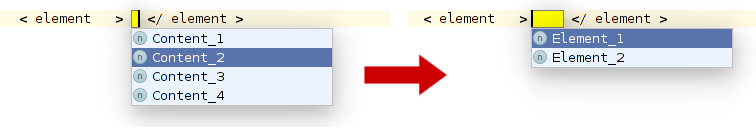
\includegraphics[scale=0.5]{./images/layer_problem.png}
	\caption{Layer problem in auto-completion}
	\label{fig:LAYERPROBLEM}
\end{figure*}

However, in order to correctly insert another nested element, a user has to perform two steps:
\begin{enumerate}
	\item Insert an object (node) of the type \mpsconcept{Content{\_}2} inside the \mpsconcept{Element{\_}1} node. The \mpsconcept{Content{\_}2} object has only a single child node of the interface type \mpsinterface{IElement}.
	\item Then, the user must trigger the auto-complete again and insert either an \mpsconcept{Element{\_}1} node or an \mpsconcept{Element{\_}2} node into the \mpsconcept{Content{\_}2} node. See the right part of Figure~\ref{fig:LAYERPROBLEM}.
\end{enumerate}
The main difficulty here is that, in the first step, the user has to (i) either correctly guess what option offered by the auto-complete menu to select, or (2) to remember the order of alternatives in the grammar rule.

Similarly, if the user would like to replace a nested \mpsconcept{Element{\_}1} node with, for example, an XML comment (represented by the \mpsconcept{Comment} node), then both intermediary layers have to be deleted before she gets back to the original selection among the concepts \mpsconcept{Content{\_}1}, $\ldots$, \mpsconcept{Content{\_}4}.

Intermediary layers have no visual appearance, and therefore it is very difficult for users to see what is actually happening and they may get confused very easily.
The layer problem is addressed by the shortcut approach, which we describe in the next subsection.

\subsubsection{The Shortcut Approach}
\label{sect:SHORTCUT}

The key idea of this approach is to skip all the intermediary layers (nodes) in the syntax tree and consider just the leaf nodes, e.g., to be directly offered to the user through the auto-completion menu.
Specifically, the \antlrparserrule{content} rule from the SimpleXML grammar, which is given in Figure~\ref{fig:CONTENTHIERARCHY} together with rules that determine the relevant fragment of the syntax hierarchy, expands ultimately into the leaf nodes that are highlighted using the bold font in Figure~\ref{fig:CONTENTEXPAND}.

\begin{figure*}[ht]
\centering
\begin{framed}
\begin{alltt}
  \antlrparserrule{content} : \antlrlexerrule{TEXT} | \antlrparserrule{element} | \antlrparserrule{comment} | \antlrlexerrule{CDATA} ;
  \antlrparserrule{element} : \antlrliteral{<} \antlrlexerrule{Name} \antlrparserrule{attrib}* \antlrliteral{>} \antlrparserrule{content}* \antlrliteral{</} \antlrlexerrule{Name} \antlrliteral{>} | \antlrliteral{<} \antlrlexerrule{Name} \antlrparserrule{attrib}* \antlrliteral{/>} ;
  \antlrparserrule{comment} : \antlrliteral{<!--} \antlrlexerrule{TEXT} \antlrliteral{-->} ;
\end{alltt}
\end{framed}
\caption{The parser rule \antlrparserrule{content} with other rules that determine the relevant fragment of the syntax hierarchy}
\label{fig:CONTENTHIERARCHY}
\end{figure*}

\begin{figure}[ht]
\begin{framed}
\textbf{Content{\_}1} (TEXT) \\
\ \ \ Content{\_}2 $\rightarrow$ \textbf{Element{\_}1} \\
\ \ \ Content{\_}2 $\rightarrow$ \textbf{Element{\_}2} \\
\ \ \ Content{\_}3 $\rightarrow$ \textbf{Comment} \\
\ \ \ \textbf{Content{\_}4} (CDATA)
\end{framed}
\caption{Leaf nodes of the parser tree fragment that has the \antlrparserrule{content} rule as its root}
\label{fig:CONTENTEXPAND}
\end{figure}

For the input that consists of a particular AST node $N$ and the grammar rule $R$ that expands $N$, the procedure implementing the shortcut approach systematically traverses the parser tree (AST) built in the earlier phases in order to identify each AST node that may appear at the end of some derivation chain starting by the rule $R$ from the node $N$.
Such nodes cannot expand further based on any rule in the grammar, and for that reason we call them \emph{end nodes}.

\begin{figure*}[ht]
\begin{framed}
\begin{alltt}
 1 FindAllPathsToEndNodes(\textit{R}):
 2   \textit{CurPath} = empty list of rules and nodes
 3   \textbf{return} FindPaths(\textit{R}, \textit{CurPath})
 4
 5 FindPaths(\textit{R}, \textit{CurPath}):
 6  \textit{Paths} = empty list
 7  \textbf{for each} alternative \textit{A} \textbf{in} rule \textit{R}:
 8    \textit{NewCurPath} = Clone(\textit{CurPath})
 9    \textbf{if} \textit{A} contains only a single element \textit{E}:
10      \textit{NewCurPath}.Add(\(N\sb{E}\)) \textbf{where} \(N\sb{E}\) is the node representing \textit{E}
11      \textit{P} = FindPaths(\(R\sb{E}\), \textit{NewCurPath}) \textbf{where} \(R\sb{E}\) is the rule that expands \textit{E}
12      \textit{Paths} = Merge(\textit{Paths}, \textit{P})
13    \textbf{else}:
14      \textit{NewCurPath}.Add(\textit{R})
15      \textit{NewCurPath}.Add(\(N\sb{A}\)) \textbf{where} \(N\sb{A}\) is the node representing \textit{A}
16      \textit{Paths}.Add(\textit{NewCurPath})
17  \textbf{return} \textit{Paths}
\end{alltt}
\end{framed}
\caption{Algorithm to find all paths to end nodes for a parser rule}
\label{fig:SHORTCUTALG}
\end{figure*}

Figure~\ref{fig:SHORTCUTALG} shows the algorithm that finds all paths to some end node from a given parser rule $R$.
The algorithm is based on recursive traversal of the parser tree.
At each level of recursion, it gathers all paths that lead from the current parser rule $R$ to some end node through its alternatives (line~7).
Two cases may occur:
\begin{itemize}
	\item When a particular alternative $A$ of the rule $R$ contains only a single element $E$, and the element is a reference to another parser rule (line 9), the alternative $A$ is an intermediary layer that can be transparently hidden from the user of the MPS language.
		  A run of the algorithm continues, at line 11, by recursively processing alternatives of the rule corresponding to $E$, which lies at the next level of the parser tree.
	\item Otherwise, an end node of a derivation chain was found and the recursion stops (lines 13-16).
\end{itemize}
By appending the node corresponding to the current alternative (lines 10 and 15) and the rule that leads to the alternative (line 14), the algorithm creates a full path that contains the target end node as the last element of the chain.

We use the name \emph{shortcut approach} for this algorithm, because the paths collected by the algorithm provide shortcuts from the given rule to end nodes, by the virtue of hiding all intermediary layers.
For example, the result of this algorithm for the \antlrparserrule{content} rule (Figure~\ref{fig:CONTENTHIERARCHY}) is the list of five items already shown in Figure~\ref{fig:CONTENTEXPAND}.

The primary use case for shortcuts is to generate options for the auto-completion menus, such that only the end nodes are offered.
Shortcuts have to be considered not only when nodes are inserted, but also when they are deleted.
In each case, the whole chain including possibly multiple intermediary AST nodes (up to the end node) must be added, respectively deleted.
When the user wants to delete some end node from the AST of a program or document written in the MPS language, the effect of an insertion must be fully reversed.

\subsection{Phase 3: Editor}
\label{sect:EDITORDEF}

Having the complete structure of the new MPS language, the next phase is to define the visual representation of all concepts (AST nodes) in the projectional editor.
As we said in Section~\ref{sect:MPS}, MPS uses a cellular system that enables the language developer to arrange the children and properties of an AST node in a table-like manner.
Cells of different types are supported by MPS --- for storing property values, references to child nodes, and keywords (string literals), and also cells that influence layout (e.g., indentation).
The specific goal of this phase is to create the Editor aspect for each language concept (element), such that all attributes of the concept --- name, properties, children --- are projected using the respective cell types.

The main problem that we had to address is the absence of information about the code layout and whitespace in the ANTLR grammar of an input language.
Rules forming the grammar only tell what the syntax tree looks like and how the program code is decomposed into AST nodes.
Here we present a solution that is only partially automated for reasons explained below.

We experimented with several heuristics to derive a useful code layout, but all of them produced rather suboptimal results.
However, we observed that the most tedious and error-prone step in the manual definition of the Editor aspect is the creation of cells for all literals (keywords), properties, children, and other fields of a given concept that should appear in its visual representation.
This step can be very easily automated.

Our solution that we implemented in the current version of the \textsc{Ingrid} method is to create all the cells and place them in a single row.
The resulting basic layout is illustrated on the example of the \mpsconcept{Element{\_}1} concept in the upper left corner of Figure~\ref{fig:EDITORADJUST}.
Further adjustments of the layout, such as indentation and line breaks, can be done very efficiently in the MPS IDE.
The bottom right part of Figure~\ref{fig:EDITORADJUST} shows a fully customized layout for the \mpsconcept{Element{\_}1} concept.

\begin{figure*}[ht]
	\centering
	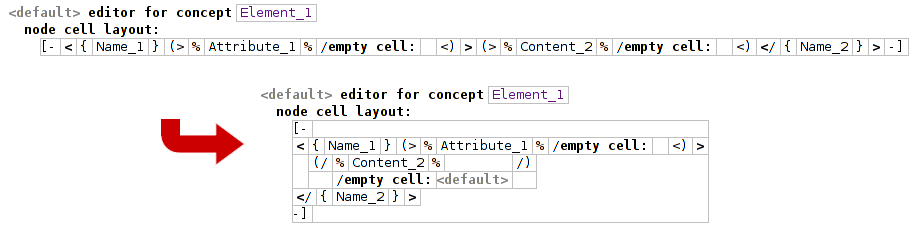
\includegraphics[scale=0.55]{./images/editor_adjustment.png}
	\caption{Editor aspect of the \mpsconcept{Element{\_}1} concept}
	\label{fig:EDITORADJUST}
\end{figure*}

Based on our experience, it takes a very short time to manually adjust the layout into a form much better than any fully automated heuristic could achieve.
We expect that a typical user of the \textsc{Ingrid} method will be able to use the projectional editor in MPS quite efficiently.
More details are provided in Section~\ref{sect:EVAL}, including our experience with several mainstream programming languages.

We have found that the combination of two steps, (1) automated placing of cells into a single row and (2) subsequent manual adjustment of the layout, is a very fast and efficient way of creating a nice code layout.
Nevertheless, we plan to work on a more automated approach to the definition of Editor aspects in the future, probably using some techniques of machine learning.
The key idea would be to derive the code layout from a set of valid input source files.
We believe that the user would have to adjust the editor manually a little bit even in this case, because the results of a machine learning-based approach would not be perfect.

\subsection{Phase 4: Text Generation}
\label{sect:TEXTGENDEF}

The purpose of the last phase of the MPS language construction is to generate the TextGen aspect for each concept.
We use the \mpsconcept{Element{\_}1} concept again for illustration.
Figure~\ref{fig:TEXTGENBASIC} shows a very basic example of BaseLanguage code that can be used as its TextGen aspect.
The code appends all literals, properties, and children of \mpsconcept{Element{\_}1} to the output buffer, and does that in the same order as they appear in the corresponding grammar rule.

\begin{figure}[ht]
\begin{alltt}
\small
\mpstgkeyword{text gen component for concept} \mpstgtarget{Element{\_}1} \{
  \mpstgparam{(context, buffer, node)->void} \{
    \mpstgaction{append} \{\mpstgliteral{<}\};
    \mpstgaction{append} \$\{\mpstgparam{node}.\mpstgnodeprop{\textit{Name}}{\_}\textit{1}\};
    \mpstgaction{append} \{\ \};
    \mpstgaction{append} \$list\{\mpstgparam{node}.\mpstgnodeprop{\textit{Attribute}}{\_}\textit{1}\};
    \mpstgaction{append} \{\mpstgliteral{>}\};
    \mpstgaction{append} \$list\{\mpstgparam{node}.\mpstgnodeprop{\textit{Content}}{\_}\textit{2}\};
    \mpstgaction{append} \{\mpstgliteral{</}\};
    \mpstgaction{append} \$\{\mpstgparam{node}.\mpstgnodeprop{\textit{Name}}{\_}\textit{2}\};
    \mpstgaction{append} \{\mpstgliteral{>}\};
  \}
\}
\end{alltt}
\caption{Basic TextGen aspect for the \mpsconcept{Element{\_}1} concept}
\label{fig:TEXTGENBASIC}
\end{figure}

Like in the case of a projectional editor, the main challenge associated with TextGen is to produce valid code with a reasonable layout.
An implementation of the TextGen aspect must determine properly where to put line breaks, indentation, and other whitespace characters.
For example, in the case of the concept representing an XML element, there must be a space between the element's name and the first attribute, while it is not required between the opening bracket \antlrliteral{\textless} and the name (Figure~\ref{fig:TEXTGENBASIC}).

Our \textsc{Ingrid} method targets mostly text-based languages, for the concepts of which the visual representation in a projectional editor must be almost equivalent to their plain-text representation.
An obvious choice would therefore be to use the same approach for Editor and TextGen.
Nevertheless, since the Editor aspect has to be adjusted manually, we decided to use a different approach for TextGen.
We designed a procedure based on a simple fully automated heuristic that provides surprisingly good results.

The procedure creates the TextGen aspect for a given language concept (AST node) in two steps.
First, it generates a basic variant that inserts spaces in between every two tokens of the textual representation of the concept.
In the second step, which is the core of our heuristic, spaces are eliminated from places where they are not really needed.
The main criterion is whether the generated plain-text output can be safely processed by a parser of the original language (using the ANTLR grammar).
We discuss all the cases here:
\begin{itemize}
	\item When there is a non-alphabetical literal that is used as a token in the grammar, and that might get recognized by the parser without the need for whitespace separators around it, then we can omit the spaces. An example of such literal is '\textless' in SimpleXML.
	\item In the case of an arbitrary string, the whitespace may be omitted when the adjacent literal ends, respectively begins, with a non-alphabetical character.
		This applies especially to the values of properties defined in Structure aspects, such as the name of an XML element.
		Based on this heuristic, redundant spaces inside of quotes will be eliminated, as well as spaces next to semicolons and around brackets.
		On the other hand, it will distinguish language keywords (e.g., \code{function}, \code{var}, \code{in}) from other literals by preserving the space character in between them.
	\item Spaces can be safely omitted also when specific optional child nodes are not present, and in the case of empty lists of child nodes, so that whitespace does not accumulate.
\end{itemize}
A space must be always inserted when two child nodes are next to each other.
Elements from a sequence of child nodes are separated with spaces or line breaks.

\begin{figure}[ht]
\begin{alltt}
\small
\mpstgkeyword{text gen component for concept} \mpstgtarget{Element{\_}1} \{
  \mpstgparam{(context, buffer, node)->void} \{
    \mpstgaction{append} \{\mpstgliteral{<}\};
    \mpstgkeyword{if} (\mpstgparam{node}.\mpstgnodeprop{\textit{Name}}{\_}\textit{1}.\textbf{isNotEmpty}) \{
      \mpstgaction{append} \$\{\mpstgparam{node}.\mpstgnodeprop{\textit{Name}}{\_}\textit{1}\};
    \}
    \mpstgkeyword{if} (\mpstgparam{node}.\mpstgnodeprop{\textit{Attribute}}{\_}\textit{1}.\textbf{size} > 0) \{
      \mpstgaction{append} \{\ \};
      \mpstgaction{append} \$list\{\mpstgparam{node}.\mpstgnodeprop{\textit{Attribute}}{\_}\textit{1} with  \};
    \}
    \mpstgaction{append} \{\mpstgliteral{>}\};
    \mpstgkeyword{if} (\mpstgparam{node}.\mpstgnodeprop{\textit{Content}}{\_}\textit{2}.\textbf{size} > 0) \{
      \mpstgaction{append} \$list\{\mpstgparam{node}.\mpstgnodeprop{\textit{Content}}{\_}\textit{2} with  \};
    \}
    \mpstgaction{append} \{\mpstgliteral{</}\};
    \mpstgkeyword{if} (\mpstgparam{node}.\mpstgnodeprop{\textit{Name}}{\_}\textit{2}.\textbf{isNotEmpty}) \{
      \mpstgaction{append} \$\{\mpstgparam{node}.\mpstgnodeprop{\textit{Name}}{\_}\textit{2}\};
    \}
    \mpstgaction{append} \{\mpstgliteral{>}\};
  \}
\}
\end{alltt}
\caption{Full TextGen aspect for the \mpsconcept{Element{\_}1} concept}
\label{fig:TEXTGENFINAL}
\end{figure}

\begin{figure}[ht]
\begin{alltt}
\small
\mpstgkeyword{if} (\mpstgparam{node}.\mpstgnodeprop{\textit{Content}}{\_}\textit{2}.\textbf{size} > 0) \{
  \mpstgaction{append} \textcolor{Blue}{\textbf{\textbackslash{}n;}}
  \mpstgaction{indent buffer;}
  \mpstgkeyword{with indent} \{
    \mpstgaction{append} \$list\{\mpstgparam{node}.\mpstgnodeprop{\textit{Content}}{\_}\textit{2} with  \};
  \}
  \mpstgaction{append} \textcolor{Blue}{\textbf{\textbackslash{}n;}}
\} 
\end{alltt}
\caption{Fragment of the TextGen aspect of \mpsconcept{Element{\_}1} with adjusted indentation}
\label{fig:TEXTGENADJUSTED}
\end{figure}

Figure~\ref{fig:TEXTGENFINAL} contains the complete, automatically generated, TextGen aspect for the \mpsconcept{Element{\_}1} concept, which represents the full SimpleXML element.
Such code may be adjusted manually very easily in order to produce nicely indented XML documents.
We only need to wrap the \mpsconcept{Content{\_}2} child node with indentation and change the sequence separator to a new line character.
A fragment of the resulting adjusted aspect (code) is in Figure~\ref{fig:TEXTGENADJUSTED}.

\subsection{Remarks about Grammars}

During our work on the \textsc{Ingrid} method, we have also observed that practical usability of a resulting MPS language depends on the specific manner in which the input ANTLR grammar is defined.
We discuss several issues and our workarounds in this section.

\paragraph{Adjusting grammars.}
In some cases, a small adjustment of the input grammar before the run of \textsc{Ingrid} might yield a better and more useful MPS language.
Here we illustrate this on two simple examples.

For the first example, we use the definition of an XML attribute in Figure~\ref{fig:XMLATTRIB}, which is taken from the original XML grammar.
The lexer rule \antlrlexerrule{STRING} actually says that quotes make a part of the attribute's value.
If the MPS language would faithfully match the grammar, the user would have to always input the leading and trailing quote together with the value in the projectional editor.

\begin{figure}[ht]
\begin{framed}
\begin{alltt}
  \antlrparserrule{attrib} : \antlrlexerrule{Name} \antlrliteral{=} \antlrlexerrule{STRING} ;
  \antlrlexerrule{STRING} : \antlrliteral{"} \antlrregex{~["]*} \antlrliteral{"}
         | \antlrliteral{\textbackslash'} \antlrregex{~[']*} \antlrliteral{\textbackslash'} ;
\end{alltt}
\end{framed}
\caption{Definition of an XML attribute}
\label{fig:XMLATTRIB}
\end{figure}

In our SimpleXML language, we adjusted the grammar easily in a way that we show in Figure~\ref{fig:XMLADJUST}.
We turned quotes into literals, ensuring that they will only appear in the projectional editor as string constant cells.

\begin{figure}[ht]
\begin{framed}
\begin{alltt}
  \antlrparserrule{attrib} : \antlrlexerrule{Name} \antlrliteral{="} \antlrlexerrule{TEXT1} \antlrliteral{"}
         | \antlrlexerrule{Name} \antlrliteral{=\textbackslash'} \antlrlexerrule{TEXT2} \antlrliteral{\textbackslash'} ;
  \antlrlexerrule{TEXT1} : \antlrregex{~["]*} ;
  \antlrlexerrule{TEXT2} : \antlrregex{~[']*} ;
\end{alltt}
\end{framed}
\caption{Adjusted fragment of the SimpleXML grammar}
\label{fig:XMLADJUST}
\end{figure}

The second example relates to a fragment of the JavaScript language, also known as ECMAScript.
%\footnote{https://github.com/antlr/grammars-v4/blob/master/ecmascript/ECMAScript.g4}.
Every statement in JavaScript needs to be terminated by a semicolon, newline, end of the file, or end of the block --- see the Figure~\ref{fig:JAVASCRIPTSTMT}, which contains the corresponding fragment of the ECMAScript grammar.
Since there are multiple options, a user would have to select one of them for each statement in the editor.
Technically, every language concept representing a statement would contain one child node of the interface type \mpsinterface{IEos}, which has to be assigned a proper object (i.e., an AST node corresponding to one of the options listed above).

\begin{figure}[ht]
\begin{framed}
\begin{alltt}
\small
\antlrparserrule{eos} : \antlrlexerrule{SemiColon} | \antlrlexerrule{EOF} | {lineBreakAhead()}? 
    | {{\_}input.LT(1).type() == \antlrlexerrule{CloseBrace}}? ;
\textcolor{gray}{// example reference to the eos rule}
\antlrparserrule{breakStmt} : \antlrlexerrule{Break} \antlrlexerrule{Identifier}? \antlrparserrule{eos} ;
\end{alltt}
\end{framed}
\caption{Statements in JavaScript}
\label{fig:JAVASCRIPTSTMT}
\end{figure}

Since MPS can differentiate between statements on the AST level, there is no need for an explicit separator.
For example, we can put each statement on a distinct line, as is usual for JavaScript code, and keep just the semicolon as a fixed literal in the projectional editor.
The \antlrparserrule{eos} rule must be changed to this form: \antlrparserrule{eos} : \antlrliteral{;}.
A small adjustment of the grammar, like this one, is a very quick solution and definitely makes the generated language more usable in MPS.
On the other hand, this adjustment of the original ANTLR grammar, performed just for the purpose of creating the MPS language, changes the grammar in such a way that it does not precisely describe the standard JavaScript language.
To ensure compatibility with JavaScript, the TextGen aspect in the MPS language should put the semicolon after each statement in the plain-text representation of a program code.

\paragraph{Breaking original grammars and parsers.}
We also want to point out a general problem with grammar adjustments that we encountered, and which all potential users of the \textsc{Ingrid} method should be aware of.
The original ANTLR grammar for an input language can be very easily changed in a way that, at first, seems harmless and valid inside MPS, but the parser generated out of the adjusted grammar stops accepting the original language.
In particular, adjustments needed to improve the resulting MPS language can break down the parser.

This problem has two main causes: (1) low-level implementation details of token matching in the ANTLR parser and (2) usage of ANTLR grammars for a different purpose (that was not expected) in our project.
Since, for practical reasons, it is very important that a parser works even for documents (programs) written according to the original grammar, adjustments have to be performed very carefully by the users of \textsc{Ingrid}.


\section{Evaluation}
\label{sect:EVAL}

We implemented the proposed \textsc{Ingrid} method as an MPS plugin that allows users to generate languages from ANTLR v4 grammars.
While most of the plugin is written in Java, small fragments of BaseLanguage code were needed to bind with the MPS API, which is used to programatically generate elements of the new language and their aspects.
The plugin uses the ANTLR library~\cite{ref:ANTLR} for parsing of ANTLR v4 grammar files, and several MPS libraries that implement the MPS API.
Our complete implementation is available at \url{https://github.com/premun/ingrid}.

For the purpose of evaluation, we applied \textsc{Ingrid} to several well-established and widely used languages, including JSON, JavaScript (ECMAScript 5.1~\cite{ref:ECMASCRIPT51}), and C\#.
MPS projects that contain definitions of all three languages are also released in the public repository (\url{https://github.com/premun/ingrid}).
In the rest of this section, we discuss our experience with application of \textsc{Ingrid} to these languages, and then we highlight few general observations.

However, first we must emphasize that MPS languages automatically produced by the \textsc{Ingrid} method, as defined in this paper, are not ready-to-use full-fledged MPS counterparts of the original input languages.
The structure of such a generated MPS language fully corresponds to the respective ANTLR grammar, but its other aspects (e.g., the Editor) have to be manually tweaked (or defined from scratch) by the end user.
\textsc{Ingrid} also does not support advanced features of MPS, such as type checking.

For each of the three languages (JSON, JavaScript, and C\#), we provide (1) its MPS definition in the form that incorporates all tweaks performed manually by authors of this paper and (2) the adjusted ANTLR v4 grammar used as input for \textsc{Ingrid}, both in the repository that contains also our implementation.

\paragraph{JSON.}
The least amount of manual adjusting after the import into MPS was needed in case of the JSON language~\cite{ref:JSON}, because it is the simplest language from all that we used for our experiments.
Specifically, the first author spent less than 20 minutes in order to get a language that is ready to use.

\paragraph{JavaScript.}
In the case of JavaScript, which is an example of a widely-used complex general purpose language, automated generating of the language definition in MPS from the ANTLR grammar\footnote{https://github.com/antlr/grammars-v4/blob/master/ecmascript/ECMAScript.g4} and subsequent manual adjusting was done in less than one hour.

We are aware of other projects that aim to create a manual port of JavaScript into MPS.
For example, there is ECMAScript4MPS~\cite{ref:ECMA4MPS} developed by the author of the PE4MPS project~\cite{ref:PE4MPS} that we described in Section~\ref{sect:RELATED}.

The main advantage of \textsc{Ingrid} over ECMAScript4MPS is that, despite its current limitations, \textsc{Ingrid} fully automatically produces the definition of JavaScript in MPS that needs just minor adjustments to be really useful.
\textsc{Ingrid} achieved a very good result especially in the case of language structure, concept aliases, and support for auto-completion.
The Structure aspect generated by \textsc{Ingrid} is very similar to that of the ECMAScript4MPS project, which was created manually over a large number of hours.

\paragraph{C\#.}
Another very complex programming language that we used for experiments is C\#~\cite{ref:CSHARP}.
Before we could run \textsc{Ingrid}, we had to manually adjust the ANTLR grammar of C\# in order to ensure that \textsc{Ingrid} produces at least a reasonable structure of the MPS language.
The Editor aspect was modified afterwards, but only for some of the concepts generated by \textsc{Ingrid}. 
Roughly one hour of manual effort was needed in total.
Nevertheless, additional modifications of the grammar and selected aspects of the MPS language (Editor, TextGen) are still needed to get an optimal result.
A great flexibility and complexity of the C\# language is the main reason behind all the necessary changes to the language definition in MPS and to the ANTLR grammar.
The definition is quite large, involving more than 800 concepts, and therefore building of the language takes a rather long time.

\paragraph{Other languages.}
We also tried to apply \textsc{Ingrid} on few other languages, such as Python and Ruby.
Results are mixed because ANTLR grammars of these languages are written in a style that is not fully compatible with \textsc{Ingrid}.
For example, the structure and hierarchy of rules in the Python grammar are quite different from JavaScript or JSON, and consequently the language definition created by \textsc{Ingrid} is rather badly organized.
We plan to address this limitation in the future.
However, significant modifications of the grammar would probably be necessary anyway.

\paragraph{General observations.}
The main overall benefit of the \textsc{Ingrid} method is partial automation.
Most of the languages discussed above, which we tried to create in MPS by using \textsc{Ingrid}, are quite complex regarding their structure and syntax variety.
Therefore, completely manual definition would be a very time-consuming and error-prone process.
Fully automated generation of the Structure aspect is where \textsc{Ingrid} spares the user from many hours of tedious and sometimes quite challenging work.

On the other hand, our experiments with complex languages show that, in the case of the Editor and TextGen aspects, manual adjustment (e.g., adding line breaks and indentation) is a very effective approach that takes only a short time --- in particular, much less time than we expected.
The first author spent between 20 and 60 minutes of work on each language, when adjusting the result of automated generation into a more useful and readable form.
MPS IDE provides good support for efficient tweaking of the code layout in Editor and TextGen, allowing users to reach optimal results very fast.
All of this justifies some of our decisions that we have described in Section~\ref{sect:EDITORDEF} and Section~\ref{sect:TEXTGENDEF}, proving that our approach is quite practical.
Despite that, we also tried to design some automated heuristics during our work on the \textsc{Ingrid} project, but so far all yield rather average results when compared to what human users can achieve efficiently instead.


\section{Conclusion and Future Work}

Our contribution is the \textsc{Ingrid} method for constructing language definitions in MPS from their grammars in the ANTLR notation.
The method is only partially automated, but nevertheless it greatly reduces the amount of manual work that developers of MPS languages have to perform.
Although we discussed all the challenges, details of our solution and general observations just in the context of ANTLR grammars and JetBrains MPS, we believe they are more general --- and in particular relevant to everyone tackling a similar problem in the field of DSLs and language workbenches.

In the future, we would like to address the remaining open problems (there are many of them) and increase the level of automation.
Our primary research goal is to investigate the usage of machine learning for the purpose of generating editors that support nice and readable code layout.
The information about code layout, once it is available, will be then leveraged and used also to improve TextGen.
Another subject for future work is generating parsers that would allow users to import existing source code into MPS.




\begin{acks}
% TODO mozna pridat jeste nejaky dalsi grant (az clanek nekam vezmou)
This work was partially supported by JetBrains.
\end{acks}


\bibliographystyle{ACM-Reference-Format}

\begin{thebibliography}{}

\bibitem{ref:MPSBOOK} F. Campagne. 2014. The MPS Language Workbench, Volume I. CreateSpace Independent Publishing Platform.

\bibitem{ref:DHL80} V. Donzeau-Gouge, G. Huet, B. Lang, and G. Kahn. 1980. Programming Environments Based on Structured Editors: The Mentor Experience. Research Report RR-0026, INRIA.

\bibitem{ref:BISONFLEX} J. Levine. 2009. Flex \& Bison: Text Processing Tools. O'Reilly Media.

\bibitem{ref:KV10} L.C.L. Kats and E. Visser. 2010. The Spoofax Language Workbench: Rules for Declarative Specification of Languages and IDEs. In Proceedings of OOPSLA 2010, ACM.

\bibitem{ref:ANTLRBOOK} T. Parr. 2013. The Definitive ANTLR 4 Reference. Pragmatic Bookshelf.

\bibitem{ref:MBEDDR} M. Voelter, D. Ratiu, B. Schaetz, and B. Kolb. 2012. mbeddr: an Extensible C-based Programming Language and IDE for Embedded Systems. In Proceedings of SPLASH 2012, ACM.

\bibitem{ref:VSB14} M. Voelter, J. Siegmund, T. Berger, and B. Kolb. 2014. Towards User-Friendly Projectional Editors. In Proceedings of SLE 2014, LNCS, 8706.

\bibitem{ref:VWK15} M. Voelter, J. Warmer, and B. Kolb. 2015. Projecting a Modular Future. IEEE Software, 32(5).

\bibitem{ref:TRFULL} P. Vysoky, P. Parizek, and V. Pech. 2018. INGRID: Creating Languages in MPS from ANTLR Grammars (Full version). Tech. Report No. D3S-TR-2018-01, Dep. of Distributed and Dependable Systems, Charles University.

\bibitem{ref:CSHARP} C\# Language Specification, Version 5.0 (2012), Microsoft Corporation, \url{https://msdn.microsoft.com/en-us/library/ms228593.aspx}

\bibitem{ref:ECMASCRIPT51} ECMAScript Language Specification, Edition 5.1 (June 2011), \url{http://www.ecma-international.org/ecma-262/5.1/Ecma-262.pdf}

\bibitem{ref:JSON} The JSON Data Interchange Format, 1st Edition (October 2013), \url{http://www.ecma-international.org/publications/files/ECMA-ST/ECMA-404.pdf}

\bibitem{ref:MPS} JetBrains MPS, \url{https://www.jetbrains.com/mps/}

\bibitem{ref:ANTLR} ANTLR parser generator, \url{http://www.antlr.org}

\bibitem{ref:ANTLR2MPS} F. Campagne. The ANTRL{\_}MPS project, \url{https://github.com/CampagneLaboratory/ANTLR_MPS}

\bibitem{ref:MPSMETABNF} DSLFoundry. The mps-metabnf project, \url{https://github.com/DSLFoundry/mps-metabnf}

\bibitem{ref:ECMA4MPS} M. Lombardo. The ECMAScript4MPS project, \url{https://github.com/mar9000/ecmascript4mps}

\bibitem{ref:PE4MPS} M. Lombardo. The PE4MPS project, \url{https://github.com/mar9000/pe4mps}

\bibitem{ref:PE} M. Lombardo. PE grammars, \url{https://github.com/mar9000/pe}

\bibitem{ref:BASELANG} MPS BaseLanguage, \url{https://confluence.jetbrains.com/display/MPSD34/Base+Language}

\end{thebibliography}

\appendix
\section{Examples of MPS Language Aspects}
\label{sect:APX} 

The first part of this appendix contains examples of core aspects for the \code{if-then-else} statement --- Structure (Figure~\ref{fig:if_statement_structure}), Editor (Figure~\ref{fig:if_editor_definition}), and TextGen (Figure~\ref{fig:if_statement_textgen}).

\begin{figure}[ht]
\vspace{-2mm}
\centering
\begin{alltt}
\small
\mpsstkeyword{concept} IfStatement \mpsstkeyword{extends} Statement
        \mpsstkeyword{implements} IContainsStatementList

  \mpsstkeyword{instance can be root:} false
  \mpsstkeyword{alias:} \mpsstalias{if}

  \mpsstkeyword{children:}
  \mpsstproperty{condition}        : Expression[\mpsstcardinality{1}]
  \mpsstproperty{ifFalseStatement} : Statement[\mpsstcardinality{0..1}]
  \mpsstproperty{ifTrue}           : StatementList[\mpsstcardinality{1}]
  \mpsstproperty{elsifClauses}     : ElsifClause[\mpsstcardinality{0..n}]
\end{alltt}
\caption{Structure aspect of the \code{if-then-else} statement}
\label{fig:if_statement_structure}
\vspace{-4mm}
\end{figure}

Figure~\ref{fig:if_editor_definition} shows an example of what the definition of the Editor aspect for the \code{if-then-else} statement might look like.
While here we indicate positions of cell borders on each line by spaces (just for illustration), MPS GUI actually uses a graphically much more appealing way of displaying the Editor aspects, which involves vertical and horizontal lines of different colors and also background colors other than white for some cells.
The symbols \verb|[-| and \verb|-]| represent layout information, which specifies mutual positioning of the contained cells (vertical, horizontal, indentation).

\begin{figure}[ht]
\vspace{-1mm}
\centering
\begin{alltt}
\small
\mpsedannotation{<default>} \mpsedkeyword{editor for concept} \mpsedtarget{IfStatement}
  \mpsedkeyword{node cell layout:}
    [-
      \mpsedkeyword{if} \textbf{(} \% conditions \% \textbf{)} [-
      \textbf{\{}
      [- \% ifTrue % -]
      \textbf{\}}
      -]
      ?[- \mpsedkeyword{else} \% ifFalseStatement \% -]
    -]
\end{alltt}
\vspace{-1mm}
\caption{Editor aspect for the \code{if-else} statement}
\label{fig:if_editor_definition}
\vspace{-2mm}
\end{figure}

TextGen aspect for each AST node (concept of the language) has to be defined using the BaseLanguage.
The definition follows a straightforward pattern --- each node outputs its textual representation into a buffer, while calling TextGen of its children nodes.
MPS calls the corresponding method on the root AST nodes of the given program.
Figure~\ref{fig:if_statement_textgen} shows an example for the \code{if-else} statement.

\begin{figure}[ht]
\vspace{-2mm}
\centering
\begin{alltt}
\small
\mpstgkeyword{text gen component for concept} \mpstgtarget{IfStatement} \{
  \mpstgparam{(context, buffer, node)->void} \{
    \mpstgaction{append} \textcolor{blue}{\textbf{\textbackslash{}n;}}
    \mpstgaction{indent buffer;}
    \mpstgaction{append} \{\mpstgliteral{if (}\} \$\{\mpstgparam{node}.\mpstgnodeprop{condition}\} \{\mpstgliteral{) \{}\};
    \mpstgkeyword{with indent} \{
      \mpstgaction{append} \$\{\mpstgparam{node}.\mpstgnodeprop{ifTrue}\};
    \}
    \mpstgaction{append} \textcolor{blue}{\textbf{\textbackslash{}n}} \{\mpstgliteral{\}}\} \$list\{\mpstgparam{node}.\mpstgnodeprop{elsifClauses}\};
    \mpstgkeyword{if} (\mpstgparam{node}.\mpstgnodeprop{ifFalseStatement}.\textbf{isNotNull}) \{
      \mpstgaction{append} \{ \mpstgliteral{else}\} \$\{\mpstgparam{node}.\mpstgnodeprop{isFalseStatement}\};
    \}
  \}
\}
\end{alltt}
\vspace{-1mm}
\caption{TextGen aspect definition for the \code{if-else} statement}
\label{fig:if_statement_textgen}
\vspace{-2mm}
\end{figure}

Figure~\ref{fig:EDITORADJUST} shows the Editor aspect for the \mpsconcept{Element{\_}1} concept --- the basic, automatically generated, layout in the upper left corner and a fully customized layout in the bottom right part.

\begin{figure*}[ht]
	\centering
	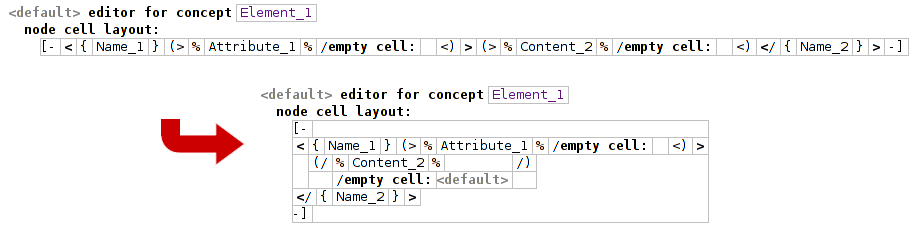
\includegraphics[scale=0.55]{./images/editor_adjustment.png}
	\caption{Editor aspect of the \mpsconcept{Element{\_}1} concept}
	\label{fig:EDITORADJUST}
\end{figure*}

Figure~\ref{fig:TEXTGENFINAL} contains the complete, automatically generated, TextGen aspect for the \mpsconcept{Element{\_}1} concept.
Such code may be adjusted by hand very easily in order to produce nicely indented XML documents.
We only need to wrap the \mpsconcept{Content{\_}2} child node with indentation and change the sequence separator to a new line character.
A fragment of the resulting adjusted code is in Figure~\ref{fig:TEXTGENADJUSTED}.

\begin{figure}[ht]
\vspace{-2mm}
\begin{alltt}
\small
\mpstgkeyword{text gen component for concept} \mpstgtarget{Element{\_}1} \{
  \mpstgparam{(context, buffer, node)->void} \{
    \mpstgaction{append} \{\mpstgliteral{<}\};
    \mpstgkeyword{if} (\mpstgparam{node}.\mpstgnodeprop{\textit{Name}}{\_}\textit{1}.\textbf{isNotEmpty}) \{
      \mpstgaction{append} \$\{\mpstgparam{node}.\mpstgnodeprop{\textit{Name}}{\_}\textit{1}\};
    \}
    \mpstgkeyword{if} (\mpstgparam{node}.\mpstgnodeprop{\textit{Attribute}}{\_}\textit{1}.\textbf{size} > 0) \{
      \mpstgaction{append} \{\ \};
      \mpstgaction{append} \$list\{\mpstgparam{node}.\mpstgnodeprop{\textit{Attribute}}{\_}\textit{1} with  \};
    \}
    \mpstgaction{append} \{\mpstgliteral{>}\};
    \mpstgkeyword{if} (\mpstgparam{node}.\mpstgnodeprop{\textit{Content}}{\_}\textit{2}.\textbf{size} > 0) \{
      \mpstgaction{append} \$list\{\mpstgparam{node}.\mpstgnodeprop{\textit{Content}}{\_}\textit{2} with  \};
    \}
    \mpstgaction{append} \{\mpstgliteral{</}\};
    \mpstgkeyword{if} (\mpstgparam{node}.\mpstgnodeprop{\textit{Name}}{\_}\textit{2}.\textbf{isNotEmpty}) \{
      \mpstgaction{append} \$\{\mpstgparam{node}.\mpstgnodeprop{\textit{Name}}{\_}\textit{2}\};
    \}
    \mpstgaction{append} \{\mpstgliteral{>}\};
  \}
\}
\end{alltt}
\caption{Full TextGen aspect for the \mpsconcept{Element{\_}1} concept}
\label{fig:TEXTGENFINAL}
\vspace{-1mm}
\end{figure}

\begin{figure}[ht]
\begin{alltt}
\small
\mpstgkeyword{if} (\mpstgparam{node}.\mpstgnodeprop{\textit{Content}}{\_}\textit{2}.\textbf{size} > 0) \{
  \mpstgaction{append} \textcolor{blue}{\textbf{\textbackslash{}n;}}
  \mpstgaction{indent buffer;}
  \mpstgkeyword{with indent} \{
    \mpstgaction{append} \$list\{\mpstgparam{node}.\mpstgnodeprop{\textit{Content}}{\_}\textit{2} with  \};
  \}
  \mpstgaction{append} \textcolor{blue}{\textbf{\textbackslash{}n;}}
\} 
\end{alltt}
\vspace{-1mm}
\caption{Fragment of the TextGen aspect of \mpsconcept{Element{\_}1} with adjusted indentation}
\label{fig:TEXTGENADJUSTED}
\vspace{-2mm}
\end{figure}



\end{document}

